\documentclass[letterpaper, 10 pt, conference]{ieeeconf}  % Comment this line out
                                                          % if you need a4paper
%\documentclass[a4paper, 10pt, conference]{ieeeconf}      % Use this line for a4
                                                          % paper

\IEEEoverridecommandlockouts                              % This command is only
                                                          % needed if you want to
                                                          % use the \thanks command
\overrideIEEEmargins
\let\labelindent\relax

% See the \addtolength command later in the file to balance the column lengths
% on the last page of the document



% The following packages can be found on http:\\www.ctan.org
\usepackage{graphics} % for pdf, bitmapped graphics files
%\usepackage{epsfig} % for postscript graphics files
%\usepackage{mathptmx} % assumes new font selection scheme installed
%\usepackage{times} % assumes new font selection scheme installed
%\usepackage{amsmath} % assumes amsmath package installed
%\usepackage{amssymb}  % assumes amsmath package installed
\let\proof\relax
\let\endproof\relax
\usepackage{amsthm}
\theoremstyle{definition}
\newtheorem{definition}{Definition}
\graphicspath{{images/}}
\usepackage{xcolor,soul}
\usepackage[inline, shortlabels]{enumitem}
\usepackage{biblatex}
\renewcommand*{\bibfont}{\small}
% personal productivity
\usepackage[colorinlistoftodos]{todonotes}
\presetkeys{todonotes}{inline}{}
\usepackage{hyperref}
\newcommand{\toread}[1]{\todo[color=red!40!white]{#1}}
\newcommand{\towrite}[1]{\todo[color=blue!40!white]{#1}}
\renewcommand{\hl}[1]{{\color{red}#1}}
\AtEveryBibitem{%
\ifentrytype{book}{
    \clearfield{url}%
    \clearfield{doi}%
    \clearfield{issn}%
    \clearfield{urldate}%
    \clearfield{review}%
    \clearfield{series}%%
}{}
\ifentrytype{collection}{
    \clearfield{url}%
    \clearfield{doi}%
    \clearfield{issn}%
    \clearfield{urldate}%
    \clearfield{review}%
    \clearfield{series}%%
}{}
\ifentrytype{incollection}{
    \clearfield{url}%
    \clearfield{doi}%
    \clearfield{issn}%
    \clearfield{urldate}%
    \clearfield{review}%
    \clearfield{series}%%
}{}
\ifentrytype{article}{
    \clearfield{url}%
    \clearfield{doi}%
    \clearfield{issn}%
    \clearfield{urldate}%
    \clearfield{review}%
    \clearfield{series}%%
}{}
\ifentrytype{inproceedings}{
    \clearfield{url}%
    \clearfield{doi}%
    \clearfield{issn}%
    \clearfield{urldate}%
    \clearfield{review}%
    \clearfield{series}%%
}{}
\ifentrytype{techreport}{
    \clearfield{url}%
    \clearfield{doi}%
    \clearfield{issn}%
    \clearfield{urldate}%
    \clearfield{review}%
    \clearfield{series}%%
}{}
\ifentrytype{misc}{
    \clearfield{url}%
    \clearfield{doi}%
    \clearfield{issn}%
    \clearfield{urldate}%
    \clearfield{review}%
    \clearfield{series}%%
}{}
}

\bibliography{rexam}

\title{\LARGE \bf
A Taxonomy for Characterizing Modes of Interactions in Goal-driven, Human-robot Teams
}
\newcommand{\citet}[1]{\citeauthor{#1}~\cite{#1}}
%\author{ \parbox{3 in}{\centering Huibert Kwakernaak*
%         \thanks{*Use the $\backslash$thanks command to put information here}\\
%         Faculty of Electrical Engineering, Mathematics and Computer Science\\
%         University of Twente\\
%         7500 AE Enschede, The Netherlands\\
%         {\tt\small h.kwakernaak@autsubmit.com}}
%         \hspace*{ 0.5 in}
%         \parbox{3 in}{ \centering Pradeep Misra**
%         \thanks{**The footnote marks may be inserted manually}\\
%        Department of Electrical Engineering \\
%         Wright State University\\
%         Dayton, OH 45435, USA\\
%         {\tt\small pmisra@cs.wright.edu}}
%}

\author{
Priyam Parashar, Lindsay M. Sanneman, Julie A. Shah, Henrik I. Christensen
}


\begin{document}



\maketitle
\thispagestyle{empty}
\pagestyle{empty}


%%%%%%%%%%%%%%%%%%%%%%%%%%%%%%%%%%%%%%%%%%%%%%%%%%%%%%%%%%%%%%%%%%%%%%%%%%%%%%%%
\begin{abstract}

As robots and other autonomous agents are incorporated into increasingly complex domains, classifying interaction in heterogeneous teams including both humans and automation is necessary. Previous literature has addressed the task of classifying human-robot interaction from different aspects and situated in different contexts. However, the factors behind an interaction work in unison and the insights from one perspective inadvertently affect the other. This motivates a need for unification of these taxonomies and framework within an upper ontology which can systematically define these relationships. In this paper we review existing taxonomies from human-robot interaction, the behavioral sciences, social taxonomies, and algorithmic taxonomies and propose an upper ontology over these works. We identify three main components characterizing interaction systems: task, environment, and team, and structure them over two levels: contextual factors and factors driven by local dynamics. Finally, we identify a classification of the effects given contextual factors and local dynamics and discuss open areas of research motivated by the observed gaps in the literature. 

\end{abstract}


%%%%%%%%%%%%%%%%%%%%%%%%%%%%%%%%%%%%%%%%%%%%%%%%%%%%%%%%%%%%%%%%%%%%%%%%%%%%%%%%

\section{INTRODUCTION}

\section{Application of the Taxonomy to Real-World Applications}
In the previous section, we introduce a taxonomy over factors impacting interaction in heterogeneous teams. These include contextual factors which cover characteristics of problem inputs, dynamics factors which include different characteristics of decisions made in terms of problem approach, and effects which are the resultant requirements on interaction given the context and dynamics. In this section we introduce a design process, drawing from the Cognitive Work Analysis (CWA) and co-active design literature, by which contextual factors can be linked to the decision of dynamics factors which in turn influence the effects. The overview of this process is depicted in figure \ref{fig:tax_design}.

    \begin{figure}[tb]
    \centering
    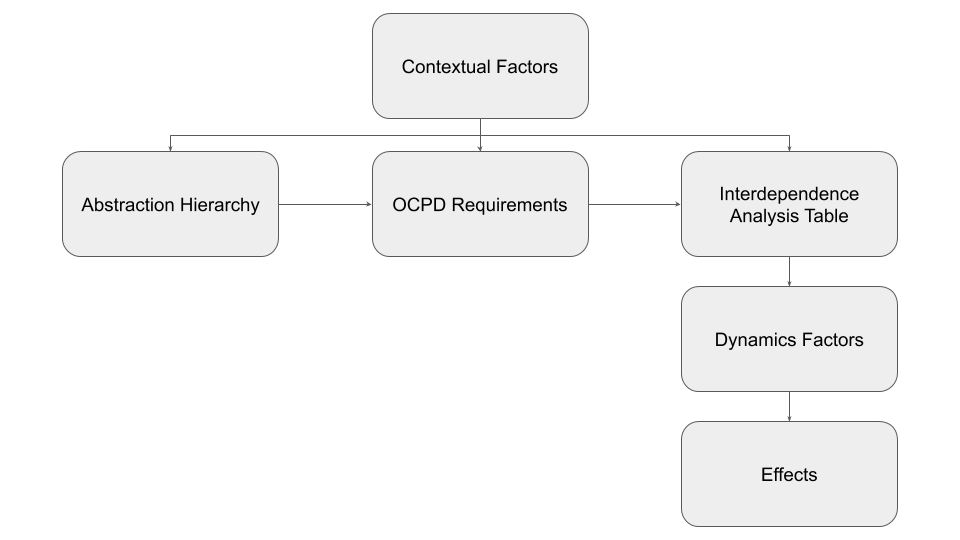
\includegraphics[width=\columnwidth]{TaxonomyDesign.png}
   \caption{Process for Determining Dynamics Factors and Effects}
    \label{fig:tax_design}
    \end{figure}

Following from work in co-active design, steps in this process include creation of an abstraction hierarchy, determination of observability, comprehensibility, predictability, and directability (OCPD) requirements, and interdependence analysis. Contextual factors act as inputs to all steps in the process, and decision of dynamics factors and effects are the outputs. We first detail each of these steps and then present three domain examples including a capture-the-flag scenario, a rover planning scenario, and an autonomous vehicle scenario to demonstrate the application of this process.

\subsection{Abstraction Hierarchy}
The CWA literature introduces the idea of an Abstraction Hierarchy (AH) for decomposition of domain goals and tasks required to support those goals for a given mission or high-level task [CITE CWA literature + applied decision science]. Goals and tasks are represented at different levels of abstraction including mission goals, priorities and values, generalized functions, and temporal functions. An example Abstraction Hierarchy for a [FILL IN] scenario is shown in Figure [FILL IN]. 

We propose development of an Abstraction Hierarchy as the first step of the analysis process for determining dynamics factors and resultant effects from the inputted contextual factors. As heterogeneous teams aim to achieve increasingly complex tasks in complex domains, different team members will need information at different levels of abstraction. The Abstraction Hierarchy provides a framework from which to determine different possible levels of abstraction of information for communication between teammates or sub-teams. 

Contextual factors inform the definition of the abstraction hierarchy at all levels. In particular, contextual task type factors including requirement type and task focus and contextual environment type factors including expected dynamics and hazard level should be considered when developing the hierarchy. Task requirement type will inform the definition of generalized functions and temporal functions, task focus will inform the definition of mission goals, priorities and vales, and functions, expected dynamics will inform the definition of temporal functions, and hazard level will inform the definition of priorities and values. 


In conjunction with analysis of observability, comprehensibility, predictability, and directability requirements and the interdpendence analysis, task allocation can be done at different levels of abstraction depending on team capabilities through consideration of the Abstraction Hierarchy. Assigning tasks at a higher level of abstraction allows teams or individuals greater flexibility in how they execute tasks, while assigning tasks at a lower level of abstraction provides teams or individuals more detailed instructions as how to how execute a task when necessary. In other words, there is a trade-off between pre-planning and flexibility in the task allocation aspect of mission planning.

\subsection{Observability, Comprehensibility, Predictability, and Directability Requirements}
[Cite co-active design] propose the consideration of observability, predictability, and directability (OPD) requirements in the determination of how a task should be structured for a joint activity. These are requirements that go beyond taskwork requirements and are necessary for the support of accomplishment of a joint activity through mutual understanding and influence between teammates. 

[Cite CAD] define observability as making pertinent aspects of one’s status, as well as one’s knowledge of the team, task, and environment observable to others. They define predictability as the need for one’s actions to be predictable enough that others can reasonably rely on them when considering their own actions. Finally, they define directability as one’s ability to direct the behavior of others and complementarily be directed by others. 

Drawing from the definition of the three levels of situational awareness in [cite Endsley], perception, comprehension, and projection, we see analogs between [CAD's] observability and predictability and [Endsley's] perception and projection, respectively. However, while comprehension is a critical component of awareness in a situation, there is currently no analog to comprehension in the OPD framework. We therefore expand on the OPD framework to additionally consider ``comprehensibility'' requirements as an additional category, giving us an OCPD framework.

We propose consideration of OCPD requirements as the second step in the analysis process for determining dynamics factors and effects. While the Abstraction Hierarchy breaks down tasks and taskwork that can be assigned at different levels of abstraction, the corresponding OCPD requirements for each task in the hierarchy determine what specific information needs to be known or communicated at each level of abstraction to support the taskwork. OCPD requirements can be defined for each box in the abstraction hierarchy to support this analysis. %maybe think about if this is the right way to do this (OCPS mayb only need to be defined for a subset)

As with the definition of the abstraction hierarchy, contextual factors inform the development of the OCPD requirements for tasks at each level of abstraction. In defining OCPD requirements, modeling contextual factors should be considered. 
%Note: need to add in something about observability requirements corresponding to both what needs to be observed and what needs to be observabile, etc 

\subsection{Interdependence Analysis}
[cite CAD] further proposes an Interdependence Analysis (IA) process to determine team decomposition and task allocation. Specifically, they introduce the concept of an IA table in which capacities required for each task and considered in conjunction with team member capabilities to determine different possible team structures for approaching a joint task (see figure [X]). While in their work, OPD requirements are derived from the connections between subtasks, we see OCPD requirements as part of the capacities required for each task as determined by the abstraction hierarchy and include them as requirements in the IA table. The output of the IA process is the enumeration of various possible team decompositions with corresponding task allocations that are feasible assignments for task execution. Drawing from the abstraction hierarchy, in this step, tasks can be considered at different levels of abstraction as necessary. 

\subsection{Tying Context to Dynamics and Effects}
The process of creating an abstraction hierarchy, determining OCPD requirements, and performing an interdependence analysis results in different possible team and task decompositions for the task that the team is aiming to accomplish. Once the team and task decomposition is determined, dynamics factors and effects can be considered. Task and goal dependencies, team roles, the expertise hierarchy, and communication are the outputs of the analysis process. The level of autonomy and level of information abstraction effects are also directly determined by the outputs of this process. 

%%TO DO: Modify the text in the above section

\subsection{Domain Examples}
In the following section we detail three examples in which we apply our analysis method to a capture the flag domain, a rover planning domain, and an autonomous vehicle domain. 
\begin{enumerate}
\item Capture the Flag Example Domain
\\In the capture-the-flag domain, we consider a scenario in which two teams each protect a flag in their own territory while attempting to capture the other team's flag in that team's territory. Team members who enter into the enemy team's territory and are tagged by an enemy team member are eliminated from the game. The first team to capture the enemy team's flag and successfully return it to their own territory win the game. We ground the capture-the-flag scenario in the RoboFlag testbed domain introduced by D`Andrea and Babish {cite}. In their setup, two teams of 6-10 robots and 2 people apiece in a hybrid simulated-physical environment are each trying to cross into the opponent’s territory, capture their flag, and return to their own territory while evading the enemy team. This domain demonstrates human-robot interaction at high speeds in dynamic, unstructured environments. Some of the challenges this domain poses are that teammates have limited sensing capabilities, there is distributed processing of information, and there are limited bandwidth capabilities.

%The operational context that we use to ground our approach is the RoboFlag testbed domain introduced by D`Andrea and Babish \cite{d2003roboflag}. This domain demonstrates human-robot interaction at high speeds in dynamic, unstructured environments and thus provides a rich context for exploration of these topics. The RoboFlag testbed emulates a capture-the-flag scenario in which two teams of 6-10 robots and 2 people apiece in a hybrid simulated-physical environment are each trying to cross into the opponent’s territory, capture their flag, and return to their own territory while evading the enemy team. In this domain, the human and robot teammates need to interact at speed in an environment with limited sensing capabilities, distributed processing of information, and limited bandwidth capabilities In our analysis, we divide this scenario into ``scout" and ``defend" stages with subteams dedicated to each stage.
%Add text and citation from the workshop paper here.
\begin{enumerate}
    \item Contextual Factors: Problem Inputs
    \begin{itemize}
        \item Task Factors:\\
        \textit{Nature - Hybrid}\\
        The nature of the capture-the-flag task is a hybrid of cognitive and physical. The team must both plan their next actions based on the current situation, and they must execute their plan in the real world. \\
        \textit{Focus - Hybrid: Area Coverage, Target Search}\\
        In the capture-the-flag domain, task focus included both area coverage and target search. Team members must cover their own territory and protect it from enemy team members and must cover the enemy territory as they search for the flag. The overall task also has a target search focus, since the team members need to search for the target enemy flag. 
        \textit{Criticality - Medium Criticality}\\
        In the capture-the-flag scenario, we assume that human safety is not threatened at any point during execution. We designate this scenario as having medium criticaility, since the tasks that team members execute are mission critical in that failure to perform any of them could jeopardize the team's ability to capture the other team's flag or protect their own flag.\\
        \textit{Objective: Speed, accuracy, something else?}
        
        \item Team Factors:\\
        \textit{Composition - Multiple heterogeneous humans to multiple homogeneous robots}\\
        In the capture-the-flag scenario, grounded in the RoboFlag setup, there are 2 humans and 6 robots. All robots have identical capbilities, and we assume that the humans have varying capabilities. \\
        \textit{Capabilities - Motion: (navigation, grasping/manipulation, speed, etc.) Sensor: Computation: Communication: (about environment, about own behavior, about other teammates)}\\
        \textit{Modeling -}\\
        
        \item Environment Factors: \\
        \textit{Spatial Distribution - Hybrid}\\
        In the capture-the-flag scenario, the spatial distribution is a hybrid of proximate and remote. For some of the subtasks in capture-the-flag, such as protecting the flag, team members are proximate. In other subtasks, such as scouting and capturing the flag in enemy territory, team members are distributed over a larger area and must communicate with some other team members remotely. \\
        \textit{Level of Cooperation - Adversarial}\\
        The capture-the-flag environment is adversarial, since team members need to contend with the enemy team.\\
        \textit{Spatial and Temporal Complexity - Unstructured and Dynamic}\\
        The environment in the capture-the-flag scenario is unstructured in that team members may encounter unmapped obstacles in the enemy territory. Further the locations and movements of enemy team members are unstructured and unknown ahead of time. The environment is also dynamic in that the locations of enemy team members and obstacles can move over time during execution. \\
       \textit{Mobility and Perception Constraints - None}\\
       In the capture-the-flag domain, we assume that all team members' full mobility and perception abilities are available and usable within the environmental context. \\
       \textit{Other Factors that might be important: stress level (maybe in Robin Murphy paper), something about cognitive load for the human? (for robot, this might relate to just whether it can handle required computation capabilities), physical load for the human (like if it's the middle of the night, might be more tired)?, }
    \end{itemize}


    \item Abstraction Hierarchy
    \\The abstraction hierarchy for the capture the flag domain is shown in figure \ref{fig:ctfah}. We have detailed the first three levels of the hierarchy including mission goals, priorities and values, and generalized functions. We also detail a subset of the total functions at the temporal functions level. %%Note: need to add this to the picture%%
    
    The high-level mission goal in this scenario is to capture the opponent team's flag while preventing the opponent team from capturing your team's flag first. At the second level, the priorities and values are to ``protect our flag'' and ``capture the other team's flag''.
    
   
    \begin{figure}[tb]
    \centering
    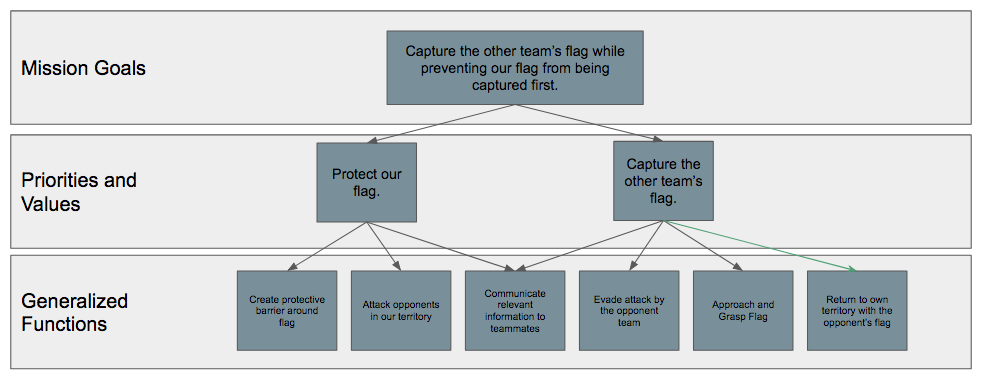
\includegraphics[width=\columnwidth]{ctfAH.png}
   \caption{Abstraction Hierarchy for Capture the Flag Scenario}
    \label{fig:ctfah}
    \end{figure}

    \item Observability, Comprehensibility, Predictability, and Directability Requirements
    \\Here we detail the definition of OCPD requirements for a subset of the boxes at each level of the hierarchy to demonstrate how such requirements can be defined and used in analysis. We further use this subset in our interdependence analysis in section d.
    
    \item Interdependence Analysis
    %Include picture of interdependence analysis table here.
    %Need to discuss team member capabilities somewhere. Maybe in the input section.
    \item Tying Context to Dynamics and Effects
    \begin{itemize}
        \item Task Factors: \\
        \textit{Planning - Hybrid}\\
        In the capture-the-flag domain, task planning is a hybrid of online planning and offline planning. The team might make an overall strategy offline, before execution, but it also needs to be able to adapt to the environment with adversarial agents online, requiring online planning. \\
        \textit{Plan-time Dependencies - Complex Dependencies}\\
        In the 
        \textit{Run-time Dependencies - }\\
        \item Team Factors: \\
        \textit{Roles- }\\
        \textit{Expertise Hierarchy - }\\
        \textit{Communication Structure - }\\
    \end{itemize}
    Task:
		Planning - online (or hybrid?)
		Plan-time Dependencies - Complex dependencies
		Run-time Dependencies - dialog-like, sense-plan-act: joint

	Team:
		Roles - Operator or peer?
		Expertise Hierarchy -
			Reconfigurability - fixed
			Decision-making protocol - distributed

		Communication Structure - Not sure


\end{enumerate}


\item Rover Planning Example Domain

\begin{enumerate}
    \item Contextual Factors: Problem Inputs
    \item Abstraction Hierarchy
    \\The abstraction hierarchy for the rover planning domain is shown in figure \ref{fig:rpah}. As with the capture the flag example, we have detailed the first three levels of the hierarchy including mission goals, priorities and values, and generalized functions. We also detail a subset of the total functions at the temporal functions level. %%Note: need to add this to the picture%%
    
       \begin{figure}[tb]
    \centering
    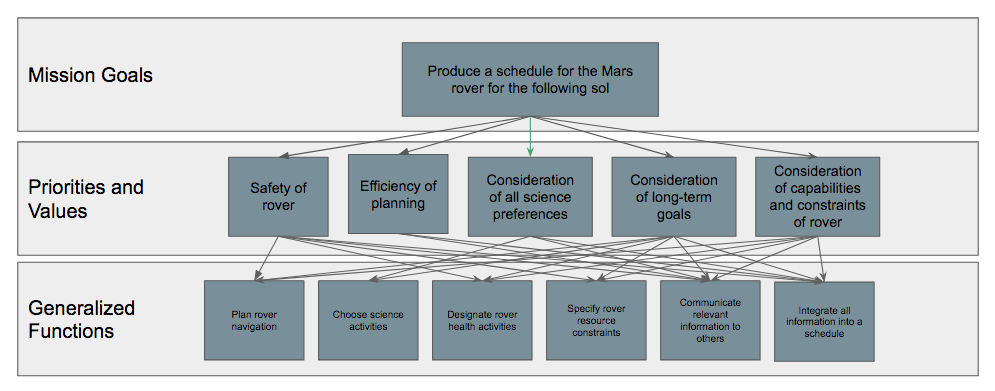
\includegraphics[width=\columnwidth]{rpAH.png}
   \caption{Abstraction Hierarchy for Rover Planning Scenario}
    \label{fig:rpah}
    \end{figure}
    
    \item Observability, Comprehensibility, Predictability, and Directability Requirements
    \item Interdependence Analysis
    \item Tying Context to Dynamics and Effects
\end{enumerate}

\item Autonomous Car Example Domain

\begin{enumerate}
    \item Abstraction Hierarchy
    \item Observability, Comprehensibility, Predictability, and Directability Requirements
    \item Interdependence Analysis
    \item Tying Context to Dynamics and Effects
\end{enumerate}

\end{enumerate}

\printbibliography


\end{document}
